\documentclass[10pt]{article}

\usepackage{spheric}
%%%TITLE
\title{Modeling of single film bubble and numerical study of the Plateau structure in foam system}
\date{}

%%AFFILIATIONS
\author[$\relax$]{Zhongguo SUN$^\dagger$}
\author[$\relax$]{Ni NI}
\author[$\relax$]{Yijie SUN}
\author[$\relax$]{Guang XI}
\affil[$\relax$]{School of Energy and Power Engineering, Xian Jiaotong University, China}
\affil[$\relax$]{\email{\dagger}{sun.zg@xjtu.edu.cn}}


%%DOCUMENT
\begin{document}

\maketitle

%\SelectedTopics{}

%%PLEASE PUT YOUR ABSTRACT HERE
\begin{abstract}
The single-film bubble has a special geometry that a certain amount of gas is shrouded by a layer of liquid film under the surface tension, which acts both on the inside and outside surfaces of the bubble. Based on the mesh-less Moving Particle Semi-implicit method (MPS), a new surface tension model was established for the single-film bubble which has double gas-liquid interfaces. Then the complex interface movement in the oscillation process of the single-film bubble was captured.

Typical flow phenomena and deformation characteristics of the liquid film were obtained by simulating and analyzing the coalescence (Fig. \ref{fig:27-1}) and connection (Fig. \ref{fig:27-2}) process of two single-film bubbles. In addition, a concave tangent method was proposed to calculate the angle of the liquid film of the connected bubbles, which could help describe the shape quantitatively.

Furthermore, the classic Plateau structure in foam system was simulated and numerically proved to be the steady statues for multi-bubble connections.

\begin{figure}[!htb]
\centering
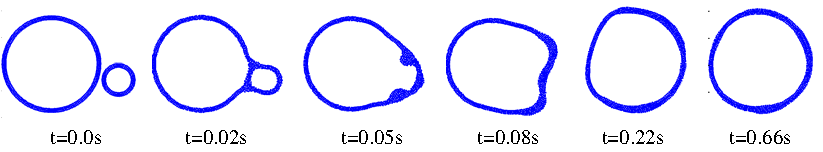
\includegraphics[width=0.95\textwidth]{27-1.pdf}
\caption{Coalescence of two single film bubbles with different sizes.}\label{fig:27-1}
\end{figure}

\begin{figure}[!htb]
\centering
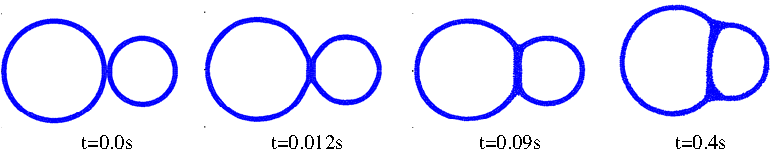
\includegraphics[width=0.95\textwidth]{27-2.pdf}
\caption{Connection of two single film bubbles with different sizes.}\label{fig:27-2}
\end{figure}

\end{abstract}


%%THE END OF ABSTRACT

\addbib

\end{document}
